\chapterimage{chapter_head_3i.jpg} % Chapter heading image

\chapter{Glossary of Oxford Terminology}

As you will have gathered if you have read this far, Oxford has much terminology which is not often heard outside its grey walls. The following is a list of a few of them.

\begin{description}
\item[Balls] Virtually every college has a ball (some smaller ones are called events). They vary greatly in scale. New College rotates hosting the commemoration ball every three years with Magdalen and Worcester. New College is hosting the commemoration ball in 2016!
\item[Battels] The bill you receive from College for the various debts you will
have incurred, i.e. drinks, chocolate, Guest Night dinners, accommodation.
\item[Black Tie Dress] \emph{Men}: dinner suit (tuxedo), though you can usually
get away with wearing a black suit, with a bow tie of any colour apart from
white; \emph{women}: stylish cocktail-length or long dress or equivalent.
\item[Blue] University award for being a jolly good sport in something like
rowing or cricket.
\item[Boat Race] The famous competition between Oxford and The Other Place (see
\emph{Cambridge}) rowing eights in London.
\item[The Bod] The Bodleian Library. Not merely the glorious building housing
the oldest library in the English-speaking world, but now something resembling a huge multinational corporation that controls all the books in Oxford.
\item[Bop] A college party.
\item[Bumps] A type of rowing race.
\item[Cambridge] A town somewhere to the north-east of Oxford where there is
another university. Commonly referred to as \emph{The Other Place}, and those
who study there are known as \emph{Tabs} (short for \emph{Cantabs}).
\item[Cherwell] A pleasant tributary of the Isis (Thames), upon which you will
spend most of your summer punting.
\item[Coming up] Opposite of going down.
\item[Cuppers] A competition between different colleges at sport.
\item[Dean's handbook] Your bible for all college related rules, to be found at
\url{http://www.new.ox.ac.uk/deans-handbook}
\item[Don] An academic.
\item[Eight] A type of boat you row.
\item[Eights week] The week in Trinity during which \emph{Summer eights} are
held.
\item[Fellow] Most academics are fellows of a college and are involved in its
governance.
\item[Fresher] A new student, whether undergraduate or grad.
\item[Front Quad] New College's oldest quad. The lodge is no longer
here, though, so it is no longer at the front\ldots
\item[Going down] Depends on the context, but it can mean to leave Oxford.
\item[High table] Where the fellows of the college eat dinner. Students may
occasionally be invited to join them. Students generally eat at common table.
\item[Hilary term] Term running from January to March. 
\item[Isis] The big river in Oxford. This is the same river that elsewhere is
called the Thames.
However, where it flows through Oxford it is called the Isis - it is incorrect to use Thames.
\item[JCR] Junior Common Room. The undergraduate body of students and their
physical common room. Graduate students are members of this.
\item[JRF] Junior Research Fellow. Similar to a post-doc. Usually funded from
the college's endowment.
\item[Long vacation] Summer vacation between June and October. 
\item[Matriculation] Ceremony where you formally become part of the university
and promise not to burn the books in the Bodleian. Done in sub fusc at the end of 1st week in Michealmas.
\item[MCR] Middle Common Room.
\item[Michaelmas] The term between October and December.
\item[New Buildings] New Buildings~(NB) are in the Holywell Quad. The porters'
lodge is there and some lecture rooms but it is mainly undergraduate accommodation.
\item[New College] The best college in Oxford. 
\item[Old buildings] Old buildings~(OB) is the name given to the staircases in
both the Front Quad and the Garden Quad.
\item[OUSU] The Oxford University Students Union.
\item[Oxford Blue] A colour.
\item[Oxford Union] Often shortened to \emph{The Union}. A world famous debating
society, connected to the university. Beer is \pounds1 a pint, and membership
fee is above \pounds200 - at least the priorities are clear.
\item[The University Parks] A large park owned by the University containing one
of the best cricket grounds in the country.
\item[Pigeon post] The internal mail. 
\item[Porters' lodge] Where you find porters, and your post (in the post room). 
\item[Proctors] Academics who are responsible for discipline and welfare across
the University.
\item[Punting] A way to move around on water and something to spend summer
doing.
\item[Quad] Short for quadrangle. A roughly square-shaped space, surrounded by
buildings. Called \emph{court} in The Other Place.
\item[Rad Cam] The Radcliffe Camera, part of the Bodleian library. 
\item[Rustication] Not quite expelled, but sent to live far away from College
while still studying at Oxford as a result of having done a bad, bad thing. 
\item[Scout] The person who cleans your room. Be very nice to them.
\item[SCR] The senior common room. Where fellows, and other senior college
officers, eat and socalise. Also a collective name for the fellows.
\item[Sent down] To be expelled. 
\item[Sub fusc] Academic dress. 
\item[Torpids] A rowing competition between colleges in Hilary. 
\item[Town] Anything or anyone not part of the University. 
\item[Trinity] The term between April and June. Also a college. 
\item[Varsity] Used to describe a sporting contest between Oxford and The Other
Place.
\item[White tie] A dress code for events which are more formal than black tie. A
couple of balls each year are white tie, including the New College ball. For men it means a dress coat and white bow tie. For women it generally means full-length ball gowns.
\item[Wykkie Bear] The MCR mascot. Add him on Facebook!
\end{description}

\begin{figure}[htbp]
\centering
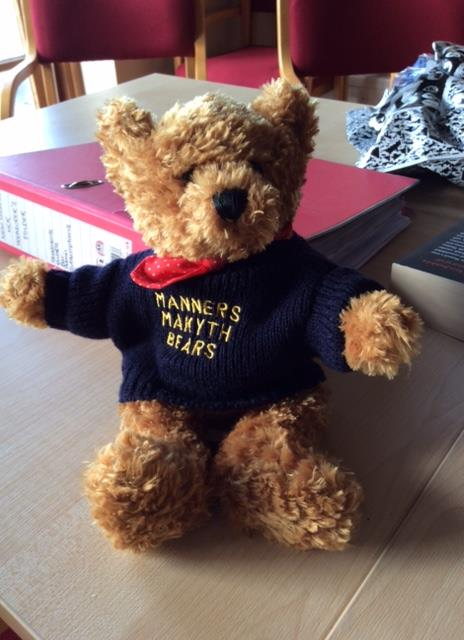
\includegraphics[width=.6\textwidth]{bear.jpg}
\caption[]{\emph{Ursus
wykehamensis collegiumnovi}, rare type of ursid, lives in the beams of
the \emph{Spoom}}
\label{fig:bear}
\end{figure}